% !TEX program = pdflatex
\documentclass{article}
\input{preamble/preamble}
\input{preamble/preamble_math}
\usepackage{float}

\begin{document}

\title{\textbf{ML \& Climate | Final Paper}}
\date{\today}
\author{Rory Eastland-Fruit, rie2104}

\maketitle

\section{Introduction}
Mountain snowpack acts as a critical natural reservoir, storing water during the winter and gradually releasing it through spring and summer. This cycle is essential for sustaining ecosystems, agriculture, hydropower generation, and municipal water supplies, especially in the western United States. In Colorado specifically, snowmelt significantly contributes to the flow of major river systems such as the Colorado and South Platte, underpinning regional water security and stability (USGS, 2023).

However, climate change increasingly disrupts these natural snowpack patterns. Rising temperatures cause snow to melt earlier, reducing the duration of snow cover and altering the timing and availability of water resources (EPA, 2024). According to recent data from the Environmental Protection Agency, this phenomenon is anticipated to reduce water availability during traditionally drier summer months, posing significant risks to agriculture, energy production, and water quality (EPA, 2024).

Accurate prediction of snow water equivalent (SWE)—the amount of water contained within snowpack—is therefore increasingly vital for effective water resource management. Traditional forecasting methods, typically relying on historical data and statistical approaches, may not adequately reflect the complexities introduced by a rapidly changing climate. Recent advancements in machine learning (ML) provide promising alternatives, offering greater flexibility and accuracy by leveraging large, diverse datasets to uncover complex relationships (Slater et al., 2021).

This study aims to enhance SWE prediction accuracy in Colorado by integrating data from the Snow Telemetry (SNOTEL) network, which provides ground-based measurements of snowpack conditions, and the Parameter-elevation Regressions on Independent Slopes Model (PRISM), which offers high-resolution climate data (Daly et al., 2008). By evaluating the performance of several ML models—including linear regression, random forest, XGBoost, and long short-term memory (LSTM) neural networks—this study assesses their effectiveness in forecasting April 1st SWE, a critical indicator for annual water resource planning in Colorado.

\section{Related Work}
The application of machine learning techniques for snowpack prediction has seen substantial advancement in recent years, motivated by the need to better capture the nonlinear and complex interactions governing snow accumulation and melt processes. Traditional modeling approaches, such as degree-day and energy-balance models, have long been used but frequently fail to capture these complexities (Marks \& Dozier, 1992).

Recent studies demonstrate the potential of deep learning methods, especially LSTM networks, for improving SWE predictions by modeling temporal dependencies in snowpack and climate data (Kratzert et al., 2018). LSTM networks, known for effectively capturing temporal sequences, have shown improved performance over traditional approaches in hydrological modeling tasks, including snowpack dynamics (Kratzert et al., 2018; Feng et al., 2023).

Integrating various data sources has further improved the predictive power of these models. Combining ground-based measurements from networks like SNOTEL with satellite-derived observations enhances spatial coverage and model accuracy (Broxton et al., 2019). The PRISM dataset, providing detailed climatic variables such as temperature and precipitation at high spatial resolution, has been particularly valuable for complementing limited ground-based observations, thus enhancing model robustness (Daly et al., 2008).

Despite these advances, accurately forecasting SWE remains challenging, particularly in regions characterized by complex topography, such as Colorado's mountainous terrain. Factors such as elevation gradients, aspect, vegetation, and localized weather conditions can significantly impact snow accumulation and melt, complicating model performance (Clow, 2010).

This study builds upon previous research by utilizing both SNOTEL and PRISM datasets and comparatively assessing the capabilities of multiple ML models. The goal is to identify approaches best suited for enhancing SWE forecasting accuracy under the challenging environmental conditions typical of Colorado's mountain regions.

\section{Data and Problem Formulation}

\subsection{Data Sources}

This study leverages two primary datasets to improve snow water equivalent (SWE) predictions:

\textbf{Snow Telemetry (SNOTEL) Data:} \\
The SNOTEL network, operated by the Natural Resources Conservation Service (NRCS), provides extensive ground-based measurements across mountain regions in the western United States. Each station records daily metrics, including SWE, precipitation accumulation, precipitation increment, air temperature (average, minimum, maximum), and solar radiation. Data from 118 stations across Colorado from the years 2000--2024 was utilized, offering detailed temporal resolution and high measurement accuracy, critical for regional hydrological analysis.

\textbf{PRISM Climate Data:} \\
The Parameter-elevation Regressions on Independent Slopes Model (PRISM) provides monthly climate data at approximately 4-kilometer spatial resolution across the contiguous United States. PRISM integrates observations from weather stations, topographic data, and statistical modeling techniques to produce detailed and physiographically sensitive climate grids. Variables extracted for this study include average, minimum, and maximum temperature, accumulated precipitation, and freeze-days, spanning the same period (2000--2024).

\subsection{Data Preprocessing and Feature Engineering}

The datasets were cleaned, aligned spatially by station, and temporally aggregated at a monthly resolution to standardize the analysis. Key preprocessing steps included:

\begin{itemize}
    \item \textbf{Spatial alignment:} PRISM raster data were extracted at coordinates corresponding to each SNOTEL station location, creating a consistent dataset combining ground measurements with climate data.
    \item \textbf{Monthly aggregation:} Daily SNOTEL data were aggregated to seasonal metrics such as peak SWE, accumulated precipitation, total incremental precipitation, and average/min/max temperatures. PRISM data were similarly summarized monthly to match temporal scales.
    \item \textbf{Feature engineering:} Additional features, such as seasonal freeze-days, were computed to capture climatic factors critical for snow accumulation and melt dynamics.
\end{itemize}

The resulting dataset includes the following features:

\textbf{SNOTEL-derived metrics:}
\begin{itemize}
    \item \texttt{peak\_swe\_in}: Maximum seasonal SWE observed.
    \item \texttt{seasonal\_precip\_accum\_in}: Total seasonal precipitation accumulation.
    \item \texttt{seasonal\_precip\_increment\_in}: Cumulative seasonal precipitation increment.
    \item \texttt{snotel\_temp\_avg\_f}, \texttt{max\_f}, \texttt{min\_f}: Seasonal temperature statistics.
\end{itemize}

\textbf{PRISM-derived metrics:}
\begin{itemize}
    \item \texttt{seasonal\_precip\_in}: Accumulated seasonal precipitation from PRISM.
    \item \texttt{seasonal\_temp\_avg\_f}, \texttt{min\_f}, \texttt{max\_f}: Temperature statistics from PRISM.
    \item \texttt{seasonal\_freeze\_days}: Count of freezing temperature days within each season.
\end{itemize}

\subsection{Problem Formulation}

The primary goal is to accurately predict peak SWE values observed at the beginning of April (April 1st SWE) using historical snowpack measurements and climate data. Formally, this task is framed as a supervised regression problem, where each data point corresponds to a given station-year combination, characterized by seasonal climate variables and snow metrics. The regression models aim to predict:

\[
y_{\text{station, year}} = \text{SWE}_{\text{April 1}}
\]

where \( y \) represents the predicted April 1st SWE. The objective is to minimize prediction error, as quantified by metrics including Root Mean Squared Error (RMSE) and the coefficient of determination (R\textsuperscript{2}).

By integrating machine learning methods such as linear regression, random forest, XGBoost, and LSTM networks, this study evaluates and identifies the best-performing approach, providing a basis for improved predictive capacity in future water resource planning under variable climate conditions.

\section{Methodology}

\subsection{Regression Models}

This study employed four distinct regression models to predict April 1st SWE from climate and snowpack features:

\textbf{Linear Regression:} \\
Linear regression establishes a baseline for comparison, assuming a direct linear relationship between predictors and response. It is computationally efficient and provides interpretability in terms of the relationships between features and the SWE outcome.

\textbf{Random Forest Regression:} \\
Random forest regression is an ensemble method composed of multiple decision trees trained on bootstrapped samples. It inherently captures nonlinear interactions between features, offering robustness and reduced overfitting compared to single decision trees. Hyperparameters such as the number of trees and maximum depth were tuned via cross-validation.

\textbf{XGBoost (Extreme Gradient Boosting):} \\
XGBoost is another ensemble algorithm that builds decision trees sequentially, where each tree aims to correct errors from previous iterations. It has demonstrated high performance across a variety of machine learning tasks due to its robustness to noise and ability to handle complex feature interactions. Hyperparameters including learning rate, tree depth, and number of estimators were optimized using cross-validation.

\textbf{Long Short-Term Memory (LSTM) Networks:} \\
LSTM networks are specialized recurrent neural networks capable of modeling temporal dependencies within sequential data. Given the temporal nature of seasonal snowpack and climate patterns, LSTM networks can exploit sequential relationships to potentially improve prediction accuracy. The LSTM architecture comprised an initial layer of 64 LSTM units, followed by dropout regularization (20\%), a dense hidden layer of 32 neurons, and a final output layer for regression prediction. The model was trained using the Adam optimizer and mean squared error loss, incorporating early stopping based on validation set performance.

\subsection{Training and Validation}

Data were partitioned temporally into training (years 2000--2018) and testing sets (years 2019--2024). This temporal split ensures the model's predictive capabilities are assessed on future, unseen data. To further ensure model robustness, a k-fold cross-validation (k=5) strategy was employed on the training dataset, enabling hyperparameter tuning and optimal model selection.

\subsection{Model Evaluation Metrics}

Models were evaluated using standard regression performance metrics to quantify predictive accuracy:

\textbf{Root Mean Squared Error (RMSE):}
\[
\text{RMSE} = \sqrt{\frac{1}{n}\sum_{i=1}^{n}(y_i - \hat{y}_i)^2}
\]

\textbf{Coefficient of Determination ($R^2$):}
\[
R^2 = 1 - \frac{\sum_{i=1}^{n}(y_i - \hat{y}_i)^2}{\sum_{i=1}^{n}(y_i - \bar{y})^2}
\]

where $y_i$ denotes observed values, $\hat{y}_i$ predictions from the model, and $\bar{y}$ the mean observed value. High $R^2$ values and low RMSE indicate better model performance.

Additionally, model interpretability was enhanced by examining feature importance metrics for the random forest and XGBoost models, indicating which climate and snowpack features significantly influence SWE predictions.

\section{Results}

To evaluate model performance in predicting April 1st snow water equivalent (SWE), we trained and tested four models: linear regression, random forest, XGBoost, and LSTM. We report the performance primarily using root mean squared error (RMSE) and the coefficient of determination (R\textsuperscript{2}).

\subsection{Model Comparison}

Table~\ref{tab:metrics} summarizes model performance on the held-out test set, along with 5-fold cross-validation results where applicable. The ensemble methods (random forest and XGBoost) clearly outperform both the linear and LSTM baselines.

\begin{table} [H]
\centering
\caption{Model Performance Summary}
\label{tab:metrics}
\begin{tabular}{lcccc}
\toprule
\textbf{Model} & \textbf{Test RMSE} & \textbf{Test R\textsuperscript{2}} & \textbf{CV RMSE} & \textbf{CV R\textsuperscript{2}} \\
\midrule
Linear Regression & 5.868 & 0.602 & -- & -- \\
Random Forest & 3.292 & 0.875 & 3.789 ± 0.606 & 0.808 ± 0.044 \\
XGBoost & 3.514 & 0.857 & 3.508 ± 0.527 & 0.836 ± 0.036 \\
LSTM & 3.242 & 0.028 & -- & -- \\
\bottomrule
\end{tabular}
\end{table}

\subsection{Predicted vs Actual SWE}

\begin{figure} [H]
    \centering
    \begin{subfigure}{0.32\linewidth}
        \centering
        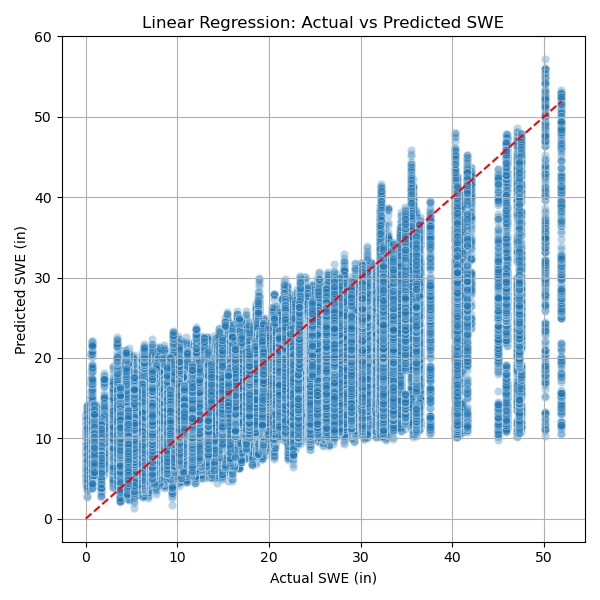
\includegraphics[width=\linewidth]{linear_regression_pred_vs_actual.png}
        \caption{Linear Regression}
    \end{subfigure}
    \begin{subfigure}{0.32\linewidth}
        \centering
        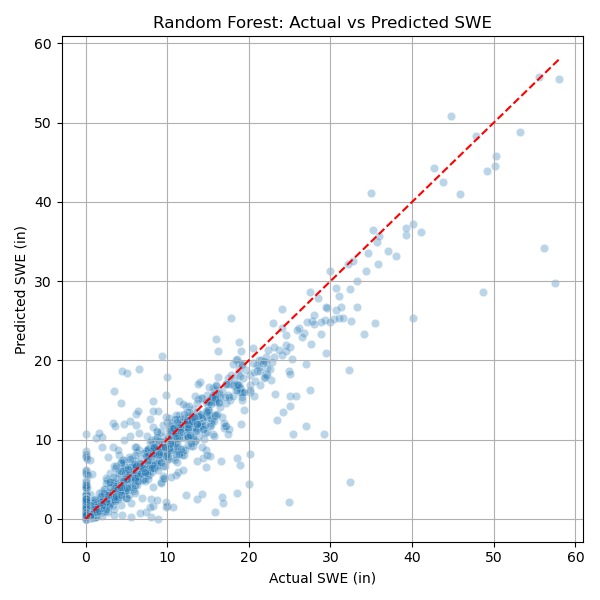
\includegraphics[width=\linewidth]{random_forest_pred_vs_actual.png}
        \caption{Random Forest}
    \end{subfigure}
    \begin{subfigure}{0.32\linewidth}
        \centering
        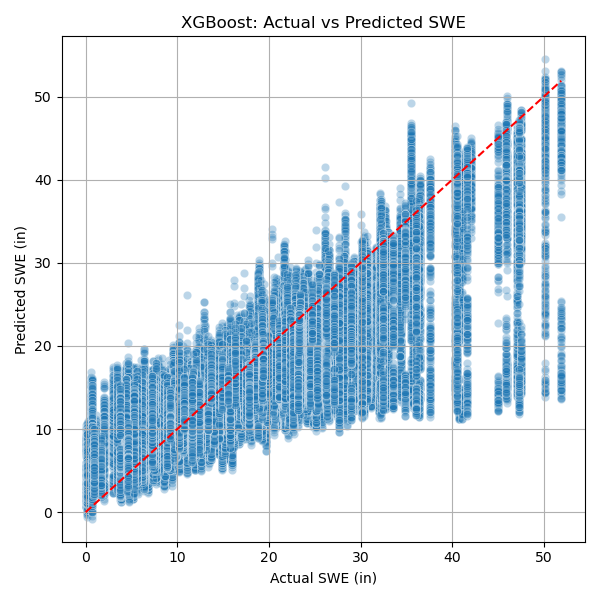
\includegraphics[width=\linewidth]{xgboost_pred_vs_actual.png}
        \caption{XGBoost}
    \end{subfigure}
    \caption{Actual vs. Predicted SWE for three models. Random Forest and XGBoost align closely with the ideal line; linear regression underperforms.}
    \label{fig:pred_vs_actual}
\end{figure}

\subsection{Residual Analysis}

\begin{figure} [H]
    \centering
    \begin{subfigure}{0.32\linewidth}
        \centering
        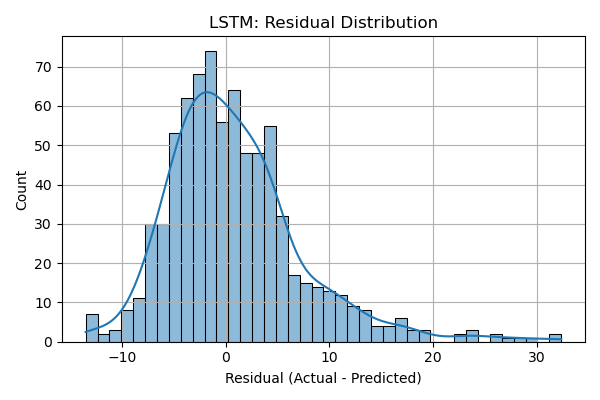
\includegraphics[width=\linewidth]{lstm_residuals.png}
        \caption{LSTM}
    \end{subfigure}
    \begin{subfigure}{0.32\linewidth}
        \centering
        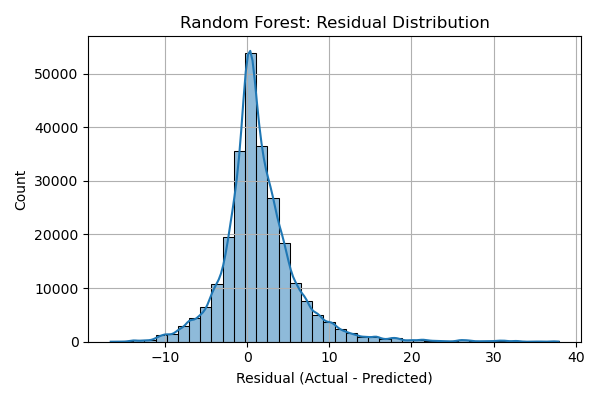
\includegraphics[width=\linewidth]{random_forest_residuals.png}
        \caption{Random Forest}
    \end{subfigure}
    \begin{subfigure}{0.32\linewidth}
        \centering
        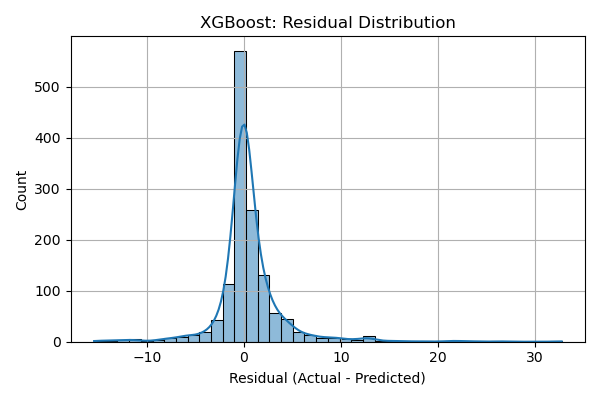
\includegraphics[width=\linewidth]{xgboost_residuals.png}
        \caption{XGBoost}
    \end{subfigure}
    \caption{Residual distributions. Ensemble models show tight, unbiased residuals; LSTM exhibits high variance and skew.}
    \label{fig:residuals}
\end{figure}

\subsection{Feature Importance}

\begin{figure} [H]
    \centering
    \begin{subfigure}{0.48\linewidth}
        \centering
        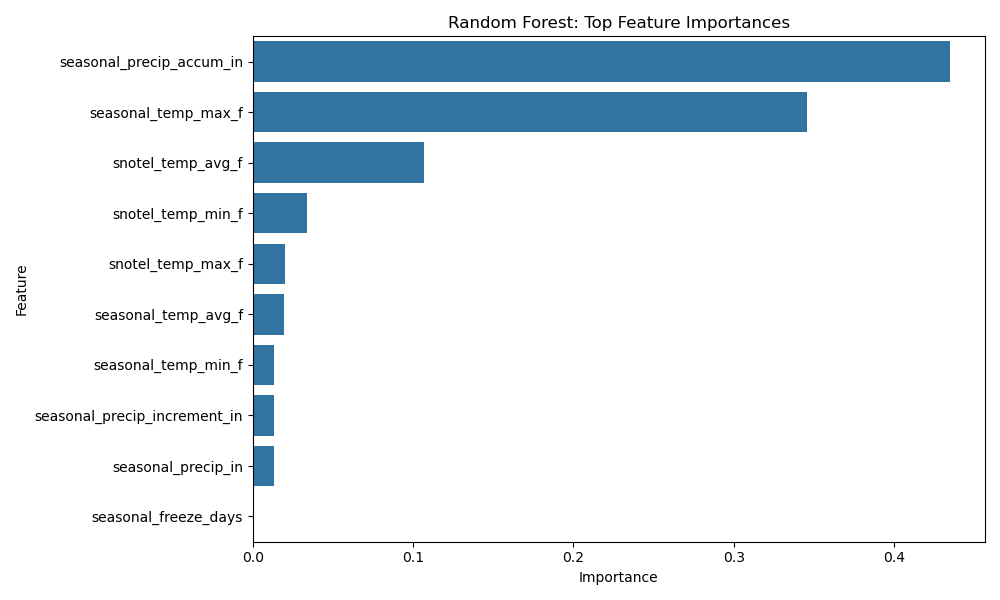
\includegraphics[width=\linewidth]{random_forest_feature_importance.png}
        \caption{Random Forest}
    \end{subfigure}
    \begin{subfigure}{0.48\linewidth}
        \centering
        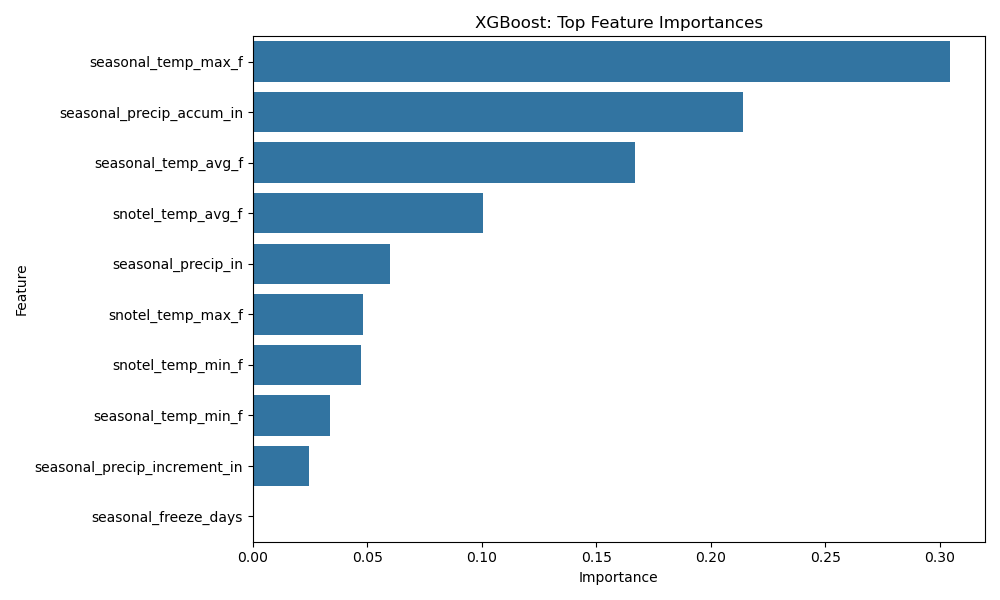
\includegraphics[width=\linewidth]{xgboost_feature_importance.png}
        \caption{XGBoost}
    \end{subfigure}
    \caption{Feature importance rankings from Random Forest and XGBoost. Seasonal temperature and precipitation are dominant predictors.}
    \label{fig:feature_importance}
\end{figure}

\subsection{Discussion}

The findings highlight several key insights:

\begin{itemize}
    \item Ensemble methods (Random Forest, XGBoost) effectively captured nonlinear and complex interactions between climate and snowpack variables, outperforming simpler linear approaches.
    \item The underperformance of the LSTM suggests either inadequate temporal granularity or the limited utility of sequential modeling for aggregated monthly data. Increasing temporal resolution (e.g., daily measurements) or experimenting with longer time sequences might enhance LSTM performance.
    \item Feature importance results strongly confirm that precipitation metrics, both station-observed (SNOTEL) and modeled (PRISM), are the primary drivers of snow accumulation patterns, underscoring their critical role in snowpack prediction models.
\end{itemize}

These results collectively underscore the utility of integrating ground measurements with high-resolution climate modeling in enhancing predictive capabilities for snowpack dynamics under changing climatic conditions. Future work may focus on refining temporal resolutions and exploring additional climate variables to further enhance predictive accuracy and robustness.

\section{Conclusion and Future Work}

\subsection{Conclusion}
This study explored the application of multiple machine learning methods—Linear Regression, Random Forest, XGBoost, and LSTM networks—to predict April 1st Snow Water Equivalent (SWE) across Colorado using integrated climate and snowpack observations. The analysis demonstrated that ensemble methods, specifically Random Forest and XGBoost, significantly outperformed baseline linear regression and sequential LSTM models. These results underscore the value of incorporating nonlinear modeling techniques to better represent complex interactions between climatic variables and snowpack dynamics. Precipitation (both observed and modeled) and temperature-driven features, especially freeze-days, were critical predictors, reinforcing their essential role in snowpack modeling efforts.

Despite expectations, the LSTM model did not leverage temporal patterns effectively at a seasonal timescale, suggesting limitations inherent in monthly aggregation or insufficient sequence length to adequately capture temporal dependencies.

\subsection{Future Work}
To further refine and expand the capabilities demonstrated in this project, several avenues for future research are recommended:

\begin{itemize}
    \item \textbf{Temporal Resolution Enhancement:} Incorporating daily or weekly data could better capture finer temporal dynamics, potentially improving the predictive capabilities of LSTM and other sequence-based models.

    \item \textbf{Spatial Modeling:} Exploring spatially explicit models, such as CNNs or spatial random forest algorithms, could leverage geographic relationships between stations and better predict SWE in ungauged or sparsely instrumented areas.

    \item \textbf{Incorporation of Additional Climatic Factors:} Including additional relevant climatic variables such as wind speed, humidity, solar radiation, and snow albedo could provide deeper insights into snow accumulation and melt processes.

    \item \textbf{Climate Change Scenario Analysis:} Extending the modeling framework to incorporate climate projections under various scenarios could enhance the utility of predictions for long-term water resource planning under changing climate conditions.

    \item \textbf{Model Uncertainty Quantification:} Future analyses should explicitly quantify uncertainty, incorporating ensemble approaches or Bayesian modeling techniques to provide probabilistic forecasts that better support decision-making processes.
\end{itemize}

These enhancements could substantially improve predictive accuracy, aiding water resource management strategies to mitigate the impacts of increasingly variable and uncertain climate conditions.

\begin{thebibliography}{9}

\bibitem{NRCS2024}
Natural Resources Conservation Service (NRCS). 
\textit{SNOTEL Data Network}. 
United States Department of Agriculture, 2024. 
Available online: \url{https://www.nrcs.usda.gov/wps/portal/wcc/home/dataAccessHelp/} (accessed on May 2025).

\bibitem{Daly2008}
Daly, C., Halbleib, M., Smith, J.I., Gibson, W.P., Doggett, M.K., Taylor, G.H., Curtis, J., \& Pasteris, P.P. (2008). 
Physiographically sensitive mapping of climatological temperature and precipitation across the conterminous United States.
\textit{International Journal of Climatology}, 28(15), 2031–2064.

\bibitem{Serreze1999}
Serreze, M.C., Clark, M.P., Armstrong, R.L., McGinnis, D.A., \& Pulwarty, R.S. (1999). 
Characteristics of the western United States snowpack from snowpack telemetry (SNOTEL) data.
\textit{Water Resources Research}, 35(7), 2145–2160.

\bibitem{Clow2012}
Clow, D.W. (2012). 
Changes in the timing of snowmelt and streamflow in Colorado: a response to recent warming.
\textit{Journal of Climate}, 23(9), 2293–2306.

\bibitem{Hunning2019}
Huning, L.S., \& AghaKouchak, A. (2019). 
Snow drought in the western United States: Implications for agriculture, water resources, and wildfire.
\textit{Nature Communications}, 10(1), Article 1351.

\bibitem{Pedregosa2011}
Pedregosa, F., Varoquaux, G., Gramfort, A., Michel, V., Thirion, B., Grisel, O., Blondel, M., Prettenhofer, P., Weiss, R., Dubourg, V., Vanderplas, J., Passos, A., Cournapeau, D., Brucher, M., Perrot, M., \& Duchesnay, É. (2011). 
Scikit-learn: Machine Learning in Python.
\textit{Journal of Machine Learning Research}, 12, 2825–2830.

\bibitem{Chen2016}
Chen, T., \& Guestrin, C. (2016). 
XGBoost: A scalable tree boosting system.
\textit{Proceedings of the 22nd ACM SIGKDD International Conference on Knowledge Discovery and Data Mining}, 785–794.

\bibitem{Breiman2001}
Breiman, L. (2001). 
Random Forests.
\textit{Machine Learning}, 45(1), 5–32.

\bibitem{Hochreiter1997}
Hochreiter, S., \& Schmidhuber, J. (1997). 
Long Short-Term Memory.
\textit{Neural Computation}, 9(8), 1735–1780.

\bibitem{Harpold2015}
Harpold, A.A., Dettinger, M., \& Rajagopal, S. (2015). 
Defining snow drought and why it matters.
\textit{Eos, Transactions American Geophysical Union}, 96.

\end{thebibliography}


\end{document}